\documentclass[10pt,letterpaper,onecolumn]{article}
\usepackage{amsmath}
\usepackage{graphicx} 
\usepackage{hyperref}
\usepackage{subfig}
\graphicspath{ {img/} }
\begin{document}
\title{Observation of Compton Scattering via Cs-137 source and Aluminum rod}
\author{
 Akhil Deshpande \\*
 Nirmal Patel \\*
 \\*
 PHY 474 Advanced Laboratory \\*
 Spring 2024 \\*
 Dr. Deepa Thomas \\*
 Department of Physics \\*
 The University of Texas at Austin \\*
 Austin, TX 78712, USA
}
\date{\today}
\maketitle
\begin{abstract}  
    $!TODO$  
\end{abstract}
\section{Introduction}
\subsection{Historical Context}
According the theory of classical electromagnetism, the wavelength of a scattered ray should be equivalent to the wavelength of the incident ray. This phenomenon is described by the theory of Thomson scattering. In 1923, Arthur Compton observed a different effect. Compton an instance in which when a high energy photon interacts with a charged particle, it releases valence electrons from the outer shell of the particle. More formally, Compton scattering is a type of scattering that is caused by the interactions between particles and waves in the X-ray to gamma ray range. \\
Energies from waves in this spectrum will usually be lower than their incident energies. This correlates to an increase in their wavelength. The amount this wavelength changes is called the Compton shift. This occurs after a relativistic, high energy photon ineracts inelastically with the charged particle. This results in an energy shift from the photon to the particle, and therefore a loss of energy exhibited by the photon.\cite{Pattison1975}
\begin{figure}
    \begin{center}
        \includegraphics*[width=3.5in]{scattering.jpg}
        \caption{This image depicts the Compton effect. An incoming X-ray is shown to have an inelastic collision with an electron, losing some of its energy. Image taken from Encyclopedia Brittanica \cite{ComptonEffectImage}.}
    \end{center}
\end{figure}
\section{Theoretical Background}
The Compton shift can be explained as a formula that is dependent on the angle of scattering:
\begin{equation}
    \label{comptonShiftWavelength} 
    \lambda' = \lambda + \frac{h}{m_e c}(1 - cos(\theta)),
\end{equation}
where 
\begin{itemize}
\item $\lambda'$ represents the wavelength after scattering, 
\item $\lambda$ represents the wavelength before scattering, 
\item $h$ is Planck's constant,
\item $m_e$ is the rest mass of the electron,
\item $c$ is the speed of light, and
\item $\theta$ is the angle of scattering.
\end{itemize}
This formula can also be expressed in terms of photon energy:
\begin{equation}
    \label{comptonShiftEnergy} 
    E_{\gamma'} = \frac{E_{\gamma}}{1 + \left( {E_{\gamma}}/{m_e c^2} \right)(1 - \cos(\theta))},
\end{equation}
where 
\begin{itemize}
\item $ E_{\gamma'}$ represents the final state photon energy, and
\item $E_{\gamma}$ represents the initial energy, 
\end{itemize}
and all other variables are as mentioned above. 
\cite{Taylor2004ModernPhysics}
These two equations are the basis for this experiment.
\section{Experimental Procedure}
\subsection{Apparatus}
\subsubsection*{Radioactive Source}
Due to the necessity of a high-energy photon source, we used a sample of Cs-137 as a radioactive gamma source. This source was fitted into a lead ball with a 1 centimeter hole drilled through the center of it. There were several lead blocks placed in front of this hole, each with the same 1 centimeter hole drilled through them. To align the source with our detector, we used a laser to ensure that the 1 centimeter hole was in like with the center of the scintillator detector. 
\subsubsection*{Scintillator}
Our scintillator was a Sodium Iodide Scintillator manufactured by Saint-Gobain. A NaI (sodium iodide) scintillator operates on the principle of scintillation, where incident gamma rays interact with the crystal lattice to produce visible light. In the context of Compton scattering, when high-energy photons collide with the electrons in the NaI crystal, part of the photon's energy is transferred to the electron, leading to the ejection of the electron and the photon's energy reduction. This process results in the excitation of atoms within the NaI crystal, which de-excite by emitting photons in the visible spectrum. These emitted photons are then detected by an adjacent photomultiplier tube (PMT), converting the light into an electrical signal proportional to the energy of the incident gamma rays. This mechanism is crucial for Compton scattering experiments, as it allows for the precise measurement of energy distributions of scattered photons, providing insights into the scattering process and the interaction of gamma rays with matter.
\subsubsection*{ORTEC Components}
We also utilized an ORTEC power supply, MCA, and a spectroscopy amplifier. The power supply was an ORTEC 556 set to 1000 Volts. This powered the ORTEC preamiplifier connected to the scintillator. The scintillator fed data to the ORTEC 672 spectroscopy amplifier. This amplifier had a shaping time of 1, an input of positive polarity on normal mode, a BLR rate of high, and a triangle shaping. This module output data to our ORTEC 927 MCA, which sorted our signals into discrete channels that correspond to the energy of the gamma rays.
\begin{figure}
    \begin{center}
        \subfloat[\centering The spectroscopy amplifier]{{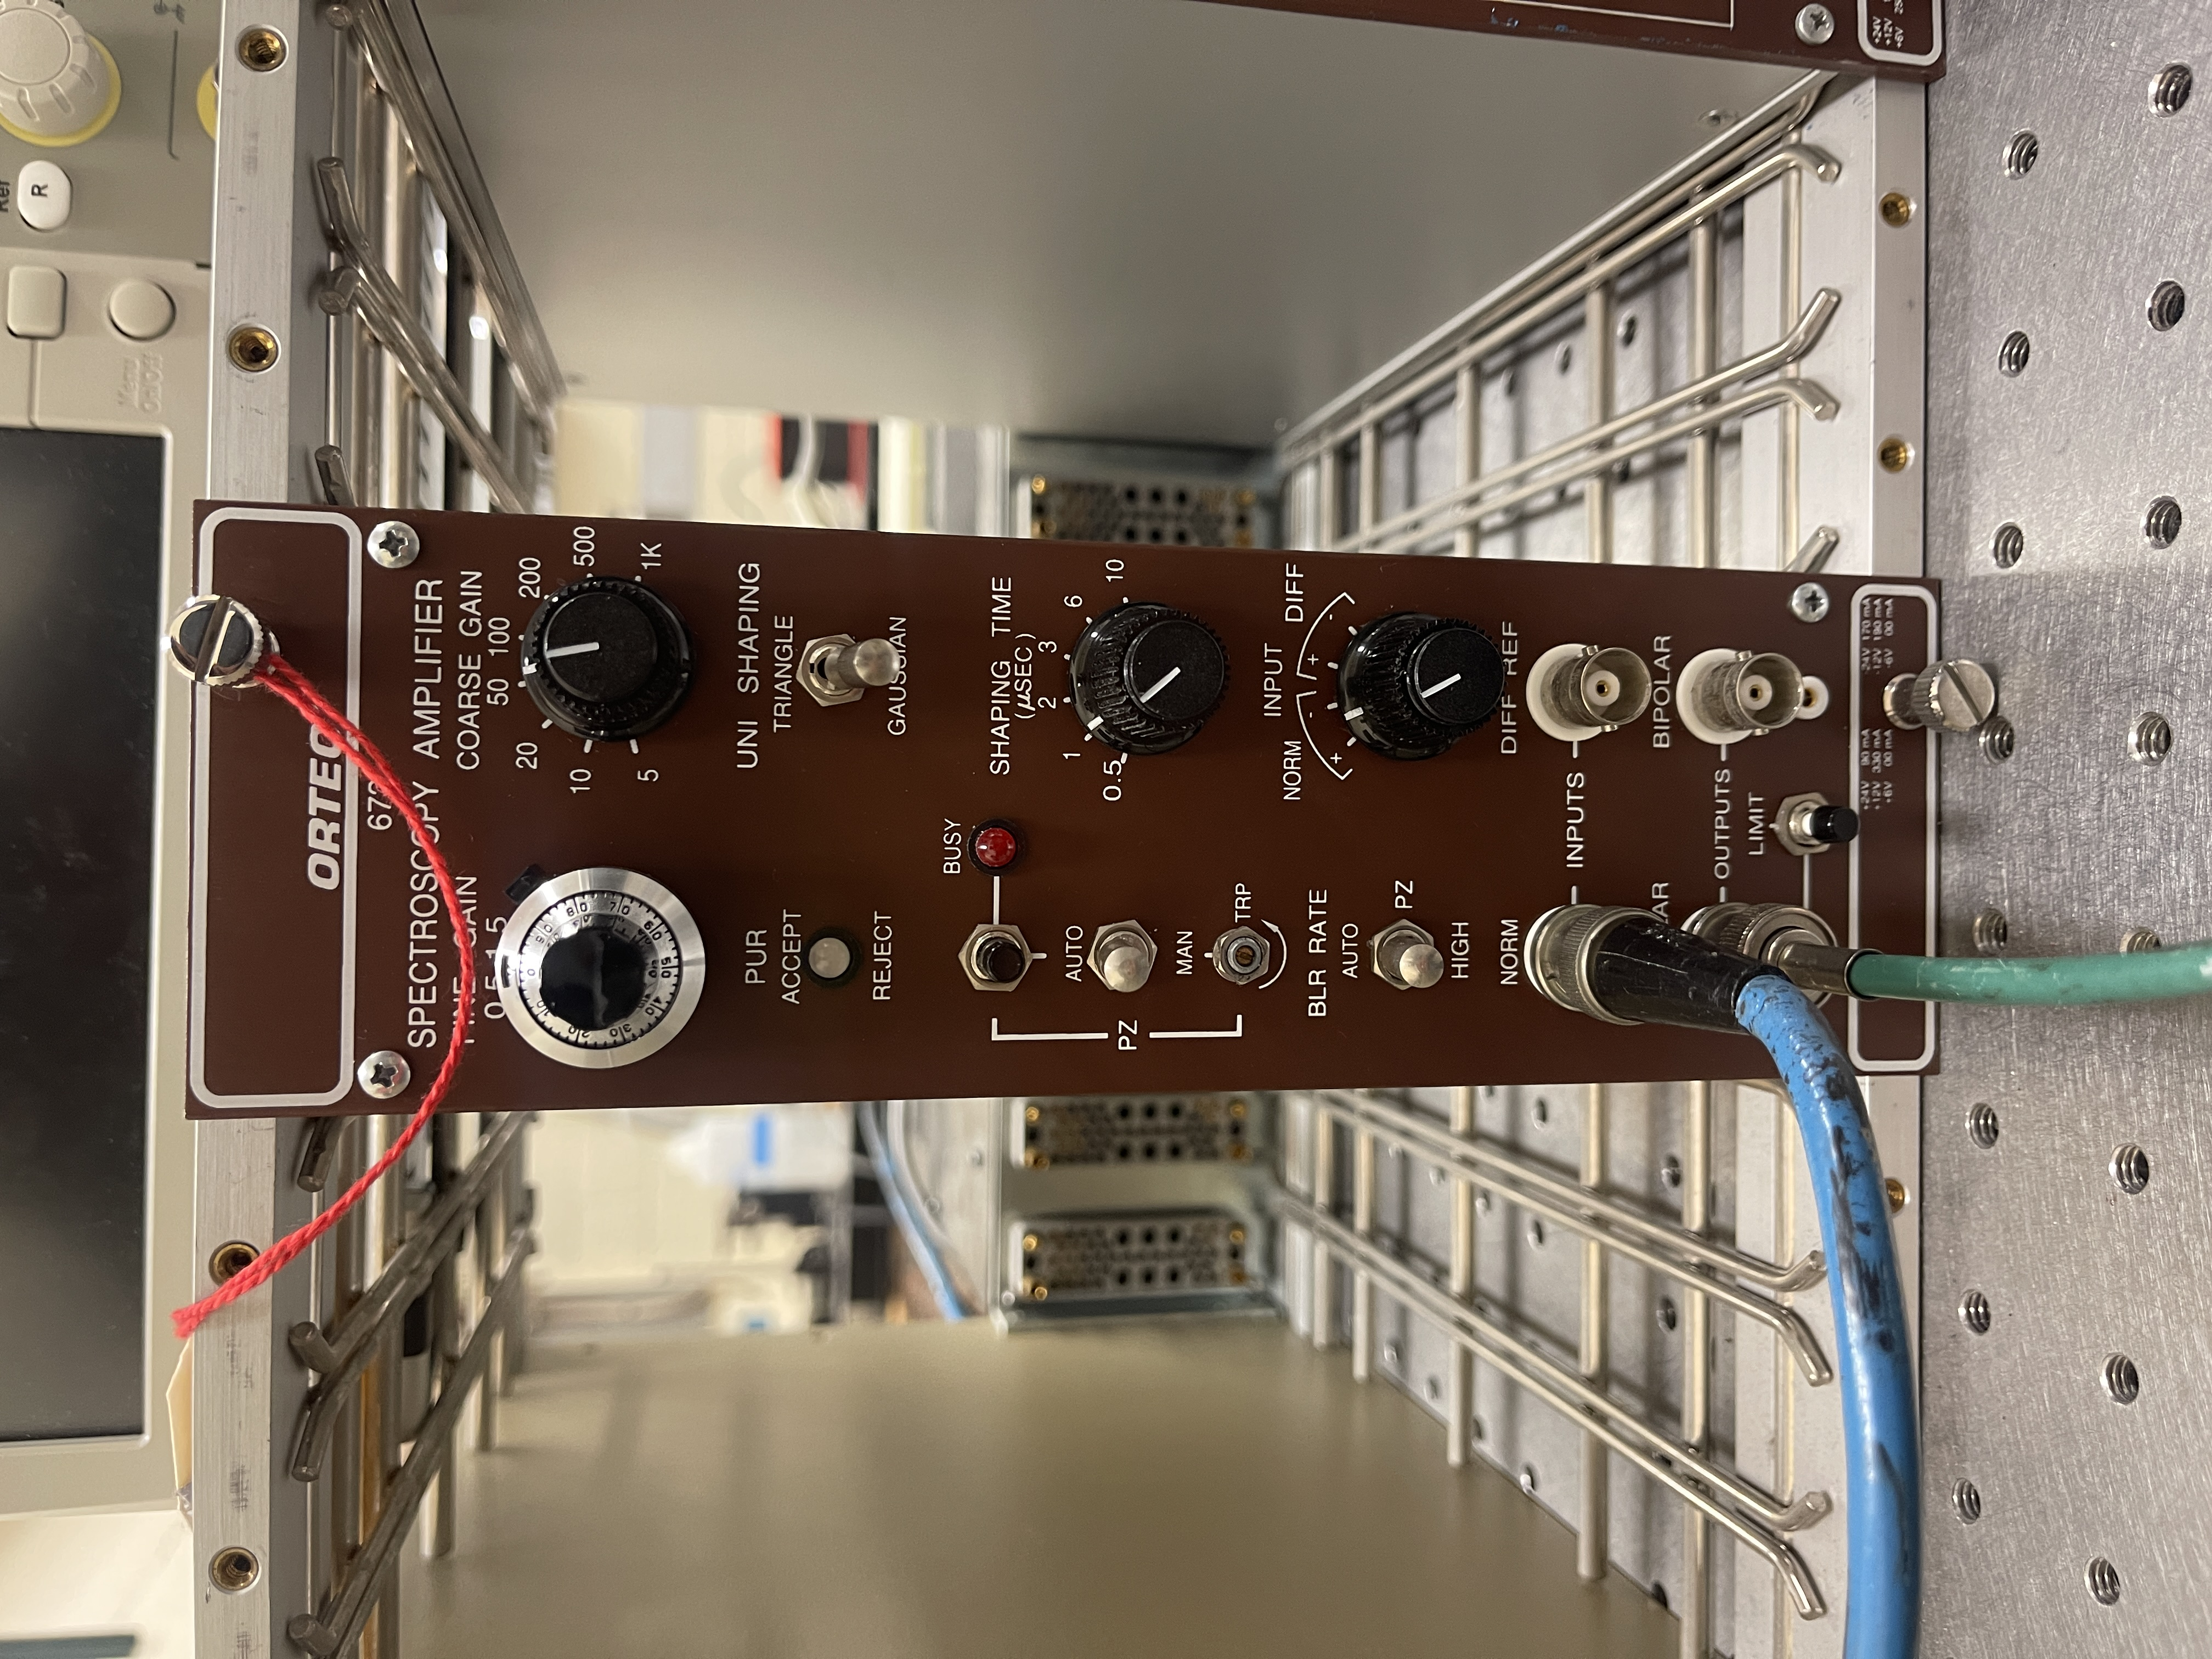
\includegraphics[width=6cm, angle = 270]{spectroscopyamplifier.JPG}}}%
        \qquad
        \subfloat[\centering The MCA and power supply]{{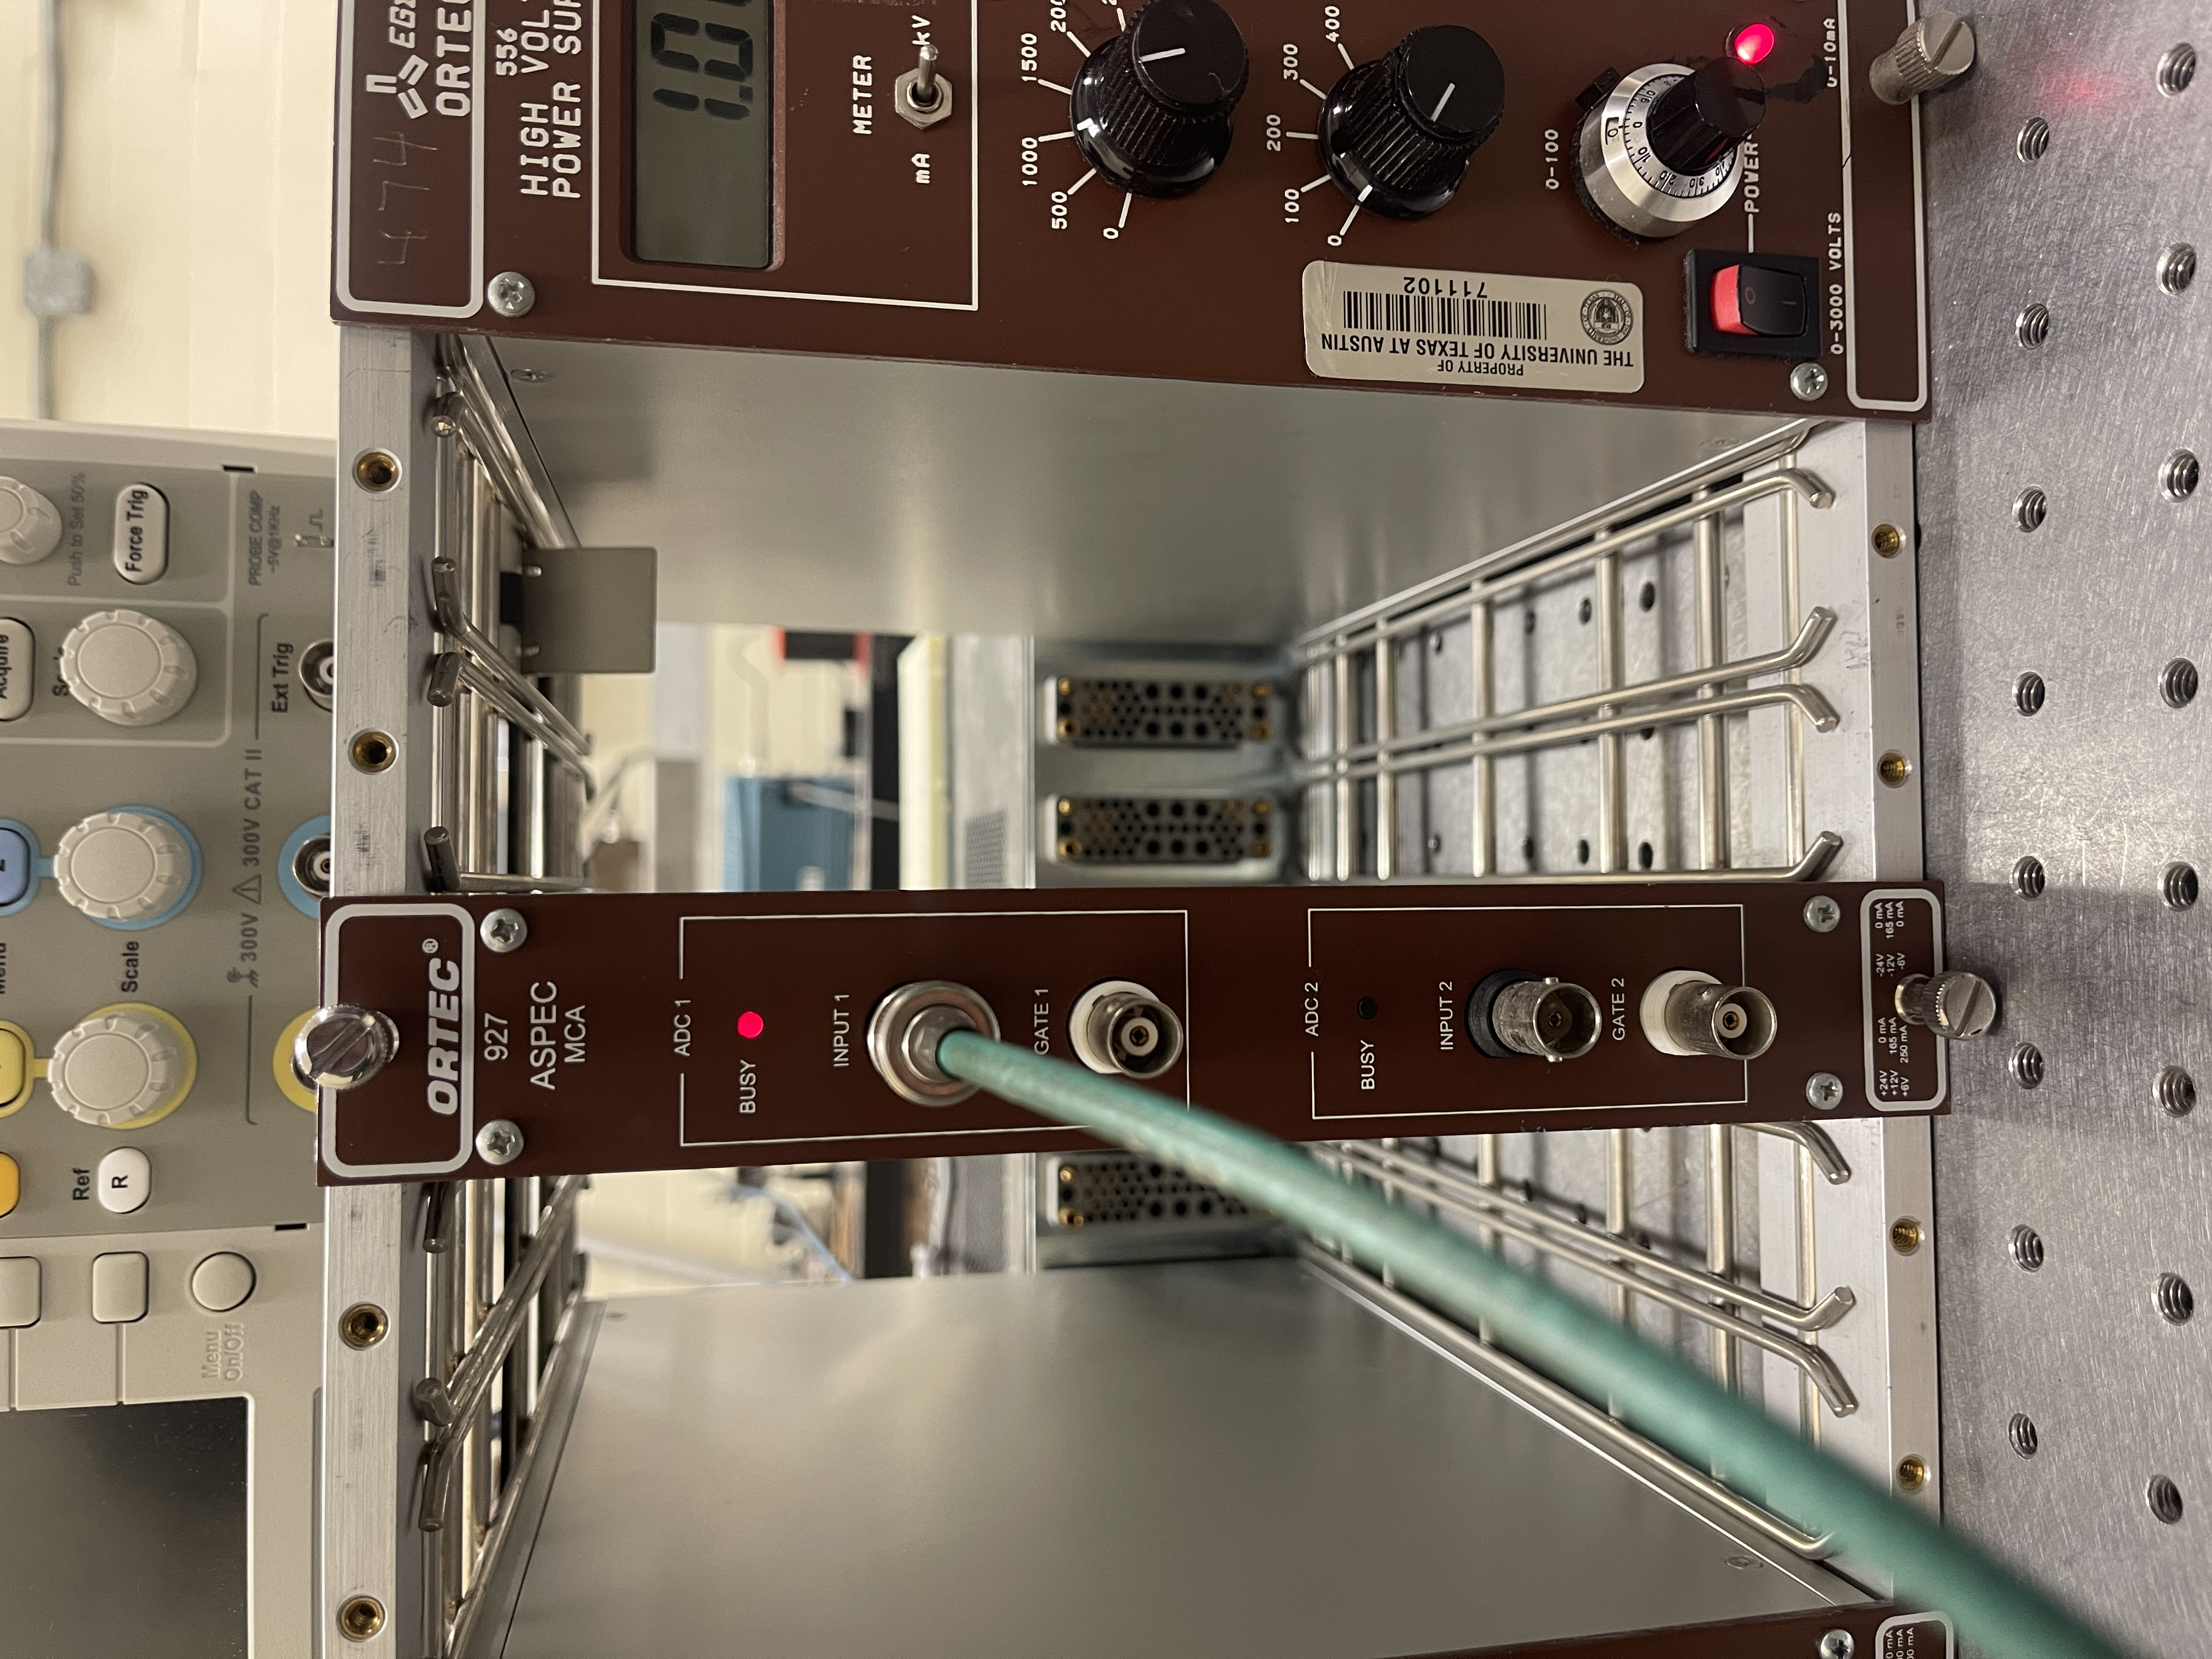
\includegraphics[width=6cm, angle = 270]{mca.JPG} }}%
        \caption{Here, we have the spectroscopy amplifier, shown on the right, and the MCA and power supply shown on the left. The settings for each are as described in the ORTEC Components subsection. For clarification, the power supply is set to 1 kV, or 1000 V.}%
        \label{fig:example}%
    \end{center}
\end{figure}
\subsubsection*{Computer Software}
We then ran trials on the lab computer's MAESTRO software. This software output data as .chn files which we used Python3 to analyze. All code and analysis functions can be found on \href{https://github.com/adeshpande03/seniorlab}{my personal github}. Furthermore, in order to make data collection easier, we created .job files which MAESTRO used to automatically save our files in case the computer turned off after being on for long periods of time. These are also found on my github.
\subsection{Data Collection}
We collected our data using MAESTRO and .job files. First, we set the scattering angle on a rotating stage. Then, we edited our .job file to reflect the amount of time, in seconds, we wanted to record data for. We then turned on the power supply and let the apparatus capture data for the set time. We did this twice per angle. Once for a run with the .5" Alumimun rod, to measure the actual scattering, and once without, to measure the background radiation of the room.
\subsection{Data Analysis}
% \section{Results}
% \section{Summary and Conclusions}
% \paragraph*{Acknowledgments}
\bibliographystyle{plain} 
\bibliography{refs} 

\end{document}

